\documentclass[11pt]{article}
\usepackage[italian]{babel}
\usepackage[utf8]{inputenc}
\usepackage{graphicx}
\usepackage{float}
\usepackage{amsmath}
\usepackage{amsfonts}
\usepackage{hyperref}
\usepackage{glossaries}
%\makeglossaries
%\newglossaryentry{magic}{
%    name={magic number},
%    description={quel numero che metti in una variabile quando è nulla ma non hai il null. Tipo -1}
%}

\usepackage[normalem]{ulem}
\newcommand{\code}[1]{\texttt{#1}}
\newcommand{\numpy}{{\tt numpy}}    % tt font for numpy
\topmargin -.5in
\textheight 9in
\oddsidemargin -.25in
\evensidemargin -.25in
\textwidth 7in
\begin{document}

% ========== Edit your name here
\author{Simone Montali\\monta.li}
\title{Riassunti di Tecnologie Internet}

\maketitle

\medskip
\section{Internet}
\subsection{HTTP}
Il \textbf{World Wide Web} è uno spazio di informazioni basato su internet, dove documenti e risorse sono identificati da indirizzi. Una \textbf{pagina web} è un documento HTML linkato ad altre pagine/risorse.
Gli \textbf{URI} (\textit{Uniform Resource Identifiers}) sono utilizzati in HTTP come mezzo identificativo delle risorse. 
\begin{center}
    \code{$schema:[//[user:password@]host[:port]][/]path[?query][\#fragment]$}
\end{center}
\textbf{HyperTezt Transfer Protocol} è un protocollo a livello applicativo, che adotta un modello client/server: uno \textbf{user agent} che inizia la connessione HTTP ed invia richieste, e un \textbf{origin server} che accetta le richieste e possiede le risorse. È inoltre utile definire altri tre termini:
\begin{itemize}
    \item \textbf{Local cache}: memoria locale (server o client)
    \item \textbf{Proxy}: applicazione intermediaria avente funzionalità server e client 
    \item \textbf{Gateway}: applicazione intermediaria che lavora per conto del server, senza renderlo noto ai client 
\end{itemize}
\subsubsection{Caratteristiche di HTTP}
\begin{itemize}
    \item \textbf{HTTP utilizza TCP}: il client inizia una connessione TCP (crea la socket) sul server, che accetta e comincia a scambiare messaggi, poi viene chiusa.
    \item \textbf{HTTP è stateless}: il server non mantiene informazioni riguardanti richieste passate 
\end{itemize}
Distinguiamo tra HTTP non-persistent, dove abbiamo un invio di risorsa alla volta, e persistent HTTP, dove più risorse vengono inviate attraverso una singola connessione TCP. Consideriamo il cosiddetto \textbf{Round Trip Time} (RTT): nella prima sono richiesti 2 RTT per risorsa (apertura connessione, invio risorsa), mentre la seconda lascia la connessione aperta, e quindi riduce il numero di RTT richieste. Inoltre, la seconda permette il \textbf{pipelining}, ossia l'invio di più richieste alla volta allo scopo di ridurre i tempi, senza attendere le risposte.
\begin{figure}[H]
    \centering
    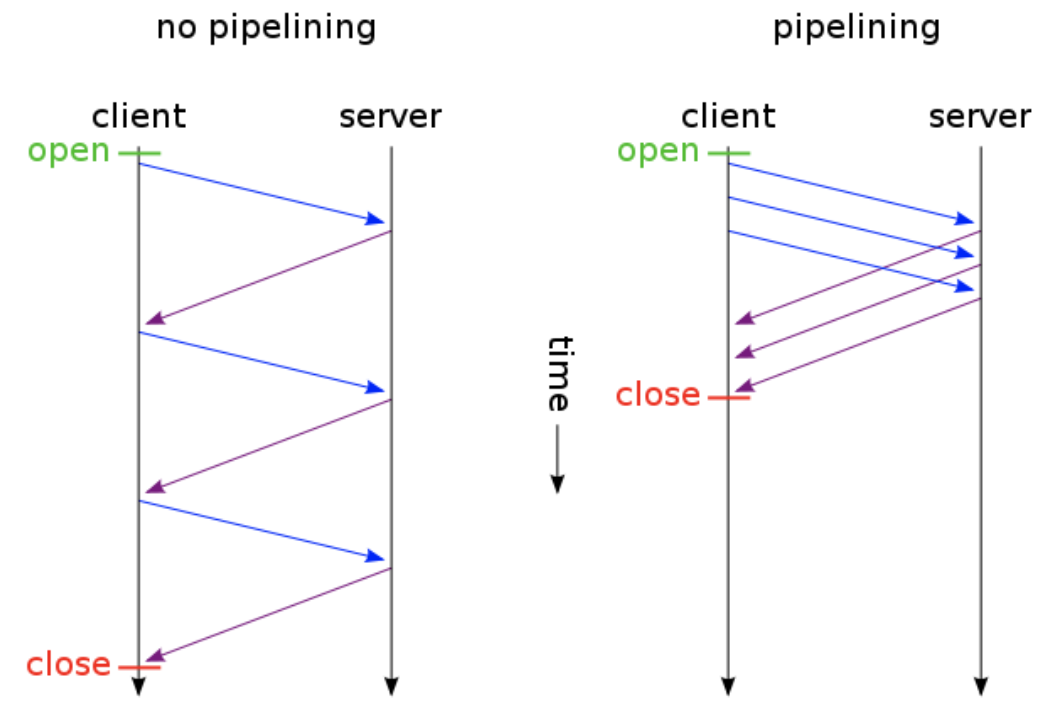
\includegraphics[width=0.6\linewidth]{res/pipelining.png}
\end{figure}
Un messaggio HTTP è formato da request/status line, header, body. Una request line è composta da \code{metodo target versioneHTTP}. Una status line è \code{versioneHTTP statusCode reasonPhrase}. Gli headers sono in formato MIME e specificano i metadati della richiesta come data, versione MIME, encoding, connessione, proxy/gateway, content-type, content-length, encoding, linguaggio, scadenza, data di modifica\dots Termina sempre con un carriage return (\code{\\r\\n}). 
\subsubsection{Metodi HTTP}
Prima di elencare i metodi, denotiamo due caratteristiche:
\begin{itemize}
    \item \textbf{Idempotenza}: significa che il metodo, chiamato più volte, restituirà sempre lo stesso risultato.
    \item \textbf{Safety}: significa che il metodo non modifica le risorse.
\end{itemize}
Procediamo elencando i metodi:
\begin{itemize}
    \item \textbf{GET}: \textit{safe ed idempotente.} Utilizzato per richiedere una risorsa, ottenuta nella risposta.
    \item \textbf{POST}: \textit{non safe, non idempotente.} Utilizzato per creare/aggiornare una risorsa. Chiamato ripetutamente, creerà più volte la risorsa.
    \item \textbf{PUT}: \textit{idempotente ma non safe.} Utilizzato per creare/aggiornare una risorsa.
    \item \textbf{DELETE}: \textit{idempotente ma non safe.} Elimina la risorsa specificata.
    \item \textbf{HEAD}: \textit{safe ed idempotente.} Come una GET ma restituisce solo l'header del messaggio.
\end{itemize}
Prima di procedere, distinguiamo le differenze tra POST e PUT: nella creazione di risorse, POST non specifica l'ID, mentre PUT si. Nell'update, POST permette di inviare la risorsa parzialmente (solo la parte da updatare), mentre PUT richiede la risorsa completa.
\subsubsection{Header delle richieste HTTP}
L'header contiene varie informazioni:
\begin{itemize}
    \item User-Agent: descrive il client che ha originato la richiesta
    \item Referer: URL della pagina che ha generato la richiesta 
    \item Host: dominio e porta a cui viene eseguita la richiesta
    \item From: indirizzo email del requester 
    \item Range: range della richiesta (utilizzato per riprendere i download)
    \item Accept, Accept-Charset, Accept-Encoding, Accept-Language: si spiega da solo; il client specifica cosa può accettare, il server decide il suo preferito
    \item If-Modified-Since, If-Unmodified-Since: permette di creare GET condizionali, ad esempio se ho una risorsa in cache e voglio verificare che sia aggiornata
    \item Authorization, Proxy Authorization 
\end{itemize}
\subsubsection{Messaggi di risposta HTTP}
La status line contiene un codice di stato:
\begin{itemize}
    \item 1xx - Informational: temporaneo mentre la richiesta viene eseguita
    \item 2xx - Successo: richiesta eseguita 
    \item 3xx - Redirection: il server ha ricevuto la richiesta ma sono necessarie altre azioni del client 
    \item 4xx - Client error: la richiesta è sbagliata
    \item 5xx - Server error: il server non è riuscito ad eseguire la richiesta 
\end{itemize}
Nell'header troviamo:
\begin{itemize}
    \item Server: stringa che descrive il server 
    \item WWW-Authenticate: contiene una challenge per il client; in caso di 401 unauthorized, il client utilizzerà la challenge per generare un codice di autorizzazione.
    \item Accept-Ranges: specifica il tipo di ranges accettabili (bytes/nulla)
\end{itemize}
\subsubsection{Cookies}
Molti siti utilizzano i cookies. Essi sono composti da 4 componenti: header line della prima risposta HTTP, header line nella prossima richiesta HTTP, file sull'host, DB sul backend del sito. 
\subsubsection{Proxy}
Il proxy è un'applicazione intermediaria che ha funzionalità server e client. Un \textbf{transparent proxy} non modifica la richiesta o risposta (es. HTTP tunneling), un \textbf{non-transparent proxy} modifica la richiesta/risposta per fornire servizi aggiuntivi.
Possiamo utilizzare un proxy server per soddisfare richieste senza coinvolgere il server originale: se la richiesta è nella cache, restituisce la risposta, altrimenti la inoltra. 
\subsection{Apache}
\textbf{Apache} nasce dal desiderio di migliorare httpd, il software server più utilizzato agli inizi di internet; è attualmente utilizzato per mantenere più del 50\% di internet. La sua architettura
 è formata da: 
 \begin{itemize}
     \item Moduli: compilati staticamente nel server o contenuti in una directory /modules o /libexec, caricata dinamicamente a runtime
    \item Apache httpd: implementa il ciclo di processamento delle richieste, composto da più fasi
    \item Multi-Processing Module: strato intermedio tra Apache e il sistema operativo, che gestisce i thread/processi
    \item Apache Portable Runtime: librerie che forniscono uno strato tra il sistema operativo e le utilities, in modo da poter essere portable
    \end{itemize}
Apache 2.0 utilizza un processo per connessione, I/O blocking. I Multi-Processing Modules bindano le porte della macchina e accettano richieste. 
\subsubsection{Configurazione}
La configurazione è eseguita tramite semplici file di testo, posizionati in varie directory e spesso divisi in più file e caricati tramite \textit{Include directives}. Una configurazione minimale richiede 5 directives:
\begin{enumerate}
    \item \code{User}: setta lo user ID con cui il server risponderà a richieste (utilizzare i permessi minimi)
    \item \code{Group}: setta il gruppo con cui il server risponderà a richieste (necessario avviare il server come root inizialmente)
    \item \code{ServerName}: setta lo schema delle richieste, hostname e porta. È in pratica l'URI.
    \item \code{DocumentRoot}: setta la directory di base delle richieste, a meno di specifiche di \textit{Alias.}
    \item \code{Listen}: setta la/le porta/e su cui accettare richieste
\end{enumerate}
In più, abbiamo:
\begin{itemize}
    \item \code{ErrorLog}: indica dove salvare il log degli errori
    \item \code{CustomLog}: indica un file dove salvare un log delle richieste, ed un filtro per decidere quali richieste loggare.
    \item \code{Include}: permette di includere altri file di configurazione
    \item \code{LoadModule}: linka una libreria/file oggetto e lo aggiunge ai moduli attivi.
    \item \code{IfModule}: permette di verificare se un modulo è installato ed eseguire directives di conseguenza.
\end{itemize}
Tramite virtual hosting possiamo hostare più siti sullo stesso server, distinguendoli in due possibili modi: tramite IP o nome. Con la seconda, non c'è necessità di IP multipli. 
Possiamo anche applicare delle configurazioni locali in determinate directory, e tramite le Options directives attivare/disattivare features, come: ExecCGI, FollowSymLinks, SymLinksIfOwnerMatch, Includes, IncludesNOEXEC, Indexes.
Inoltre, è possibile utilizzare i file \code{.htaccess} per definire cambiamenti alla configurazione in directories: inseriamo il file in una cartella e tutte le modifiche alla configurazione verranno eseguite lì e nelle subfolders. Tramite la \code{AllowOverride} della configurazione, decidiamo quali directives possono essere overridate dagli htaccess. Per migliorare le performance di Apache, il sistemosta può modificare le opzioni di Apache: è però sconsigliabile usare spazio di swap (RAM virtuale). Infine, con la directive \code{ErrorDocument}, specifichiamo cosa fare quando si incorre in un errore HTTP specifico, con 4 possibilità: messaggio hardcoded di errore (default), messaggio custom, redirect interno, redirect esterno.
\subsubsection{Avvio di Apache}
Su \href{https://www.youtube.com/watch?v=dFUlAQZB9Ng}{sistemi Unix} httpd viene eseguito come daemon continuamente; se la directive Listen è sulla porta 80, è necessario avviare Apache come root perché è una porta speciale (poi verranno lanciati child processes). Lanciamo Apache con l'\code{apachectl} control script, che setta le variabili ENV necessarie e poi avvia httpd. Se l'avvio è succesful, il server viene detacchato dalla console (scusate). Si può usare apachectl per terminare Apache, o killare il daemon.
\subsection{HTML}
Il web è basato su tre risorse: gli URI, i protocolli, e HTML. \textbf{HTML} è un linguaggio universale che permette la creazione di documenti con formattazioni, contenuti, link, design. Nasce dalla mente di Tim Berners-Lee e conta attualmente 5 versioni major, la cui ultima è 5.2. Per promuovere l'interoperabilità, ogni documento HTML deve specificare il suo character set, formato da repertorio e code positions. Inoltre, va specificato l'encoding nell'header delle richieste HTTP. Distinguiamo tra 3 parti: una linea di versione HTML, un header, un corpo. Nell'header possiamo trovare varie tipologie di tag: \code{TITLE}, \code{BASE}, \code{LINK}, \code{SCRIPT}, \code{STYLE}, \code{META}. Nel corpo, possiamo trovare DIV (block-level) e SPAN (inline). Un heading descrive l'argomento della sezione che introduce (H1..H6 in base all'importanza). Abbiamo anche alcuni tag per il testo: \code{BR} va a capo, \code{P} delimita un paragrafo, \code{PRE} delimita un testo preformattato, \code{EM}, \code{STRONG}, \code{CITE}, \code{DFN}, \code{CODE}, \code{SAMP}, \code{KBD}, \code{VAR}, \code{ABBR}, \code{ACRONYM}, \code{BLOCKQUOTE}, \code{Q}, \code{SUB}, \code{SUP}. Possiamo creare liste: \code{UL} (\textit{Unordered List}), \code{OL}(\textit{Ordered List}), \code{DL}(\textit{Definition List}). Possiamo creare tabelle: \code{TABLE, TR, TD}. Possiamo spaziarle utilizzando \code{rowspan} e \code{colspan}, captionarle con \code{CAPTION}. Possiamo creare links con il tag \code{A}, avente attributi \code{href} e \code{target}(\_blank, \_self, \_parent, \_top). Dando ID agli elementi HTML possiamo cercarli tramite gli anchor link (\#riferimento). Con l'elemento \code{IMG} embeddiamo immagini definite nell'attributo \code{src}. Con \code{OBJECT} definiamo oggetti come risorse, applets, plugin. Con i frame possiamo generare views multiple; un frame ha head, frameset e body, con attributi rows e cols. Possiamo anche creare forms, che contengono contenuto, markup, controlli, labels e li inviano ad un'action (tramite GET o POST). In HTML5 sono stati inoltre definiti nuovi tag, semantici (header, footer, article, section) , di controllo (numeri, date, orari, calendari, range), grafici (svg, canvas), multimediali (audio, video). Non sono più supportati i frames, sostituiti dagli iframes.
\subsection{CSS}
HTML non è nato per contenere tag di definizione di stile, ma piuttosto per mostrare dati. Quando cominciarono a venire aggiunti tag di stile ad HTML 3.2, come \code{font}, \code{color}, si capì che non poteva funzionare. Il World Wide Web Consortium (W3C) creò quindi \textbf{Cascading File Sheets} (CSS). In HTML4, tutta la formattazione poté quindi essere definita separatamente dall'HTML, dando la possibilità di modificare l'intero sito con un solo sito web. 
\subsubsection{Sintassi}
La sintassi consiste in un selettore, seguito da varie dichiarazioni:
\begin{center}
    \code{h1 \textbraceleft}
    \code{color:blue;}
    \code{font-size:12px;}
    \code{\textbraceright}
\end{center}
Il selector punta all'elemento HTML desiderato, mentre nel blocco di dichiarazione inseriamo una o più dichiarazioni separate da ;.
I selettori possono indicare una tipologia HTML, come \code{p}, una classe, come \code{.rowDiv}, un ID, come \code{\#title}. Possiamo includere CSS in tre modi:
\begin{itemize}
    \item Style sheet esterno: \code{<LINK rel="stylesheet" type="text/css" href="file.css">}
    \item Style sheet interno: \code{<STYLE> body\textbraceleft\textbraceright</STYLE>}
    \item Inline: \code{<H1 style="color:blue;">}
\end{itemize}
\subsubsection{Attributi notevoli}
Alcuni attributi importanti:
\begin{itemize}
    \item \textbf{Background}: background-color, background-image, background-repeat, background-attachment, background-position
    \item \textbf{Text}: color, text-align, text-decoration, text-transform, text-indent
    \item \textbf{Fonts}: permette di definire una font family (generica o specifica) con sistema fallback: le prova in ordine finché non trova la funzionante; è quindi meglio partire con specifica e terminare con generica. Oltre a font-family, abbiamo font-style (italic, oblique), font-size, font-weight
    \item \textbf{Links}: possiamo applicare ogni CSS property, ed in più abbiamo 4 selector speciali (A:link, A:visited, A:hover, A:active)
    \item \textbf{Lists}: possiamo settare i marker delle liste, o addirittura immagini come item markers con list-style-image 
    \item \textbf{Tables}: possiamo specificare i borders tramite la proprietà border, e anche width/height. Inoltre, anche text-align e vertical-align sono disponibili.
\end{itemize}

\subsubsection{Box model}
In CSS sfruttiamo il \textit{pattern} del box model: essenzialmente è ciò che wrappa un contenuto, che ci permette di aggiungere padding, bordi, margini. 
\begin{figure}[H]
    \centering
    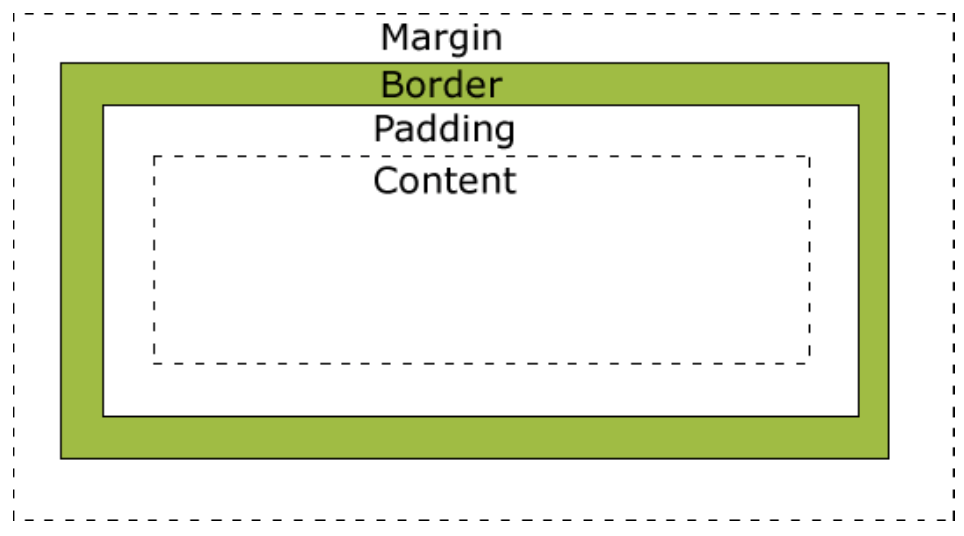
\includegraphics[width=0.6\linewidth]{res/boxmodel.png}
\end{figure}
\subsection{XML}
Sembrerà un linguaggio inutile e passato (perché lo è), ma nella sezione SOA ci sono ben due lezioni che si basano su sto schifo. \textit{Ocio.} XML sta per \textbf{eXtensible Markup Language} e serve per trasportare informazioni, non per presentarli (come HTML). I tag non sono definiti in uno standard, ma dall'utente. Possiamo, per esempio sfruttare XML per separare i dati variabili da HTML. 
\paragraph{Quando usare XML?} XML semplifica il salvataggio e la condivisione di dati, essendo un formato standard basato su testo. Semplifica i cambiamenti di piattagorma, essendo testo semplice. Tra i linguaggi scritti in XML, citiamo SVG, WSDL, RSS.
\subsubsection{Struttura}
Il documento XML inizia con il prologo, che definisce la versione XML. Comincia poi l'albero, che ha una root e delle leaves. I figli sullo stesso livello sono detti siblings (fratelli). Tutti i figli possono avere un contenuto e degli attributi. In XML è illegale omettere il tag di chiusura (tranne ovviamente nel prologo). I tag XML sono \textbf{case sensitive}. Gli attributi devono essere sempre tra virgolette. I commenti sono come in HTML: \code{<!-- Commentino -->}. XML non tronca gli spazi bianchi come HTML, e salva le nuove linee come \code{LF}. Bisogna stare attenti ad alcuni caratteri, come $<$, che vanno escapati con sequenze specifiche: \&gt;, \&amp, \&apos, \&quot;. Gli elementi XML devono seguire alcune regole di nomenclatura:
\begin{itemize}
    \item Case sensitivity
    \item Inizio con lettera o underscore
    \item Non si può iniziare con "XML"
    \item Possono contenere lettere, numeri, trattini, underscore, punti
    \item Non possono contenere spazi 
    \item Le lettere accentate non sono un problema (ma occhio ai software)
\end{itemize}
Gli attributi solitamente forniscono informazioni che non sono parte dei dati, ad esempio, se avessimo un contenuto file, l'attributo potrebbe essere il filetype. Alcuni problemi degli attributi:
\begin{itemize}
    \item Non possono contenere valori multipli
    \item Non possono contenere alberi 
    \item Non sono facilmente espansibili
\end{itemize}
Per evitare conflitti di nomi, possiamo utilizzare dei prefissi di namespace con l'attributo xmlns:
\begin{verbatim}
<h:table xmlns:h="http://www.w3.org/TR/html4/"> 
    <h:tr>
        <h:td>Apples</h:td>
        <h:td>Bananas</h:td>
    </h:tr>
</h:table>
\end{verbatim}
Dopo aver definito un namespace, tutti i contenuti con quel prefisso verranno collegati al namespace. Definire un namespace di default è utile: ci evita di utilizzare prefissi in tutti i children. 
Possiamo utilizzare anche caratteri internazionali: è però importante specificare l'encoding nel prolog. 
\subsubsection{Validità e document types}
Un documento XML corretto è detto \textit{ben formato}. Un documento XML valido deve essere compatibile ad una \textbf{document type definition}. Ne abbiamo due diverse: DTD (\textit{Document Type Definition}) e XML Schema (\textit{basata su XML}). Usiamo questi document type per vari scopi: decidere standard, verificare dati dall'esterno, verificare dati nostri. XML non lo richiede per forza, ma in ambienti di produzione ci vuole. Lo scopo di un DTD è definire la struttura, con una lista di elementi validi. Possiamo anche usarlo per definire caratteri speciali e stringhe di caratteri. L'\textbf{XML Schema} è un'alternativa basata su XML a DTD.

\subsection{JSON}
\textit{Finalmente.} JSON è il cugino che ce l'ha fatta di XML. Sta per \textbf{JavaScript Object Notation}, ed è come XML una sintassi per salvare e scambiare dati, più leggera e semplice di XML. Dal momento che JSON è proprio il modo di definire oggetti in JavaScript, non necessita di parser. Similarità con XML: self-describing, gerarchico, portable, fetchabile con una XMLHttpRequest. Differenze con XML: niente tag di chiusura, più breve, più veloce, presenza di arrays. La sintassi di JSON è derivata da JS: i dati sono accoppiati nome/valore, separati da virgole, oggetti delimitati da \textbraceleft\textbraceright, arrays delimitati da $[]$. Un valore JSON può essere un numero, stringa, boolean, array, oggetto, null.
\end{document}